% \documentclass[twocolumn]{aastex6}
\documentclass{aastex6}

\newcommand{\radmc}{\texttt{RADMC-3D}}
\newcommand{\kms}{ \textrm{km s}^{-1} }
\newcommand{\todo}[1]{ \textcolor{red}{#1}}
\newcommand{\vt}{ {\bm \theta}}
\newcommand{\msun}{M$_\odot$}

\begin{document}

\title{GW Ori: A Massive Stellar Systems with a Circumtriple Disk, Caught at Young Ages}
\author{I.~Czekala\altaffilmark{1}, S.~M.~Andrews\altaffilmark{1}, E.~L.~N.~Jensen\altaffilmark{2}, K.~G.~Stassun\altaffilmark{3,4}, G.~Torres\altaffilmark{1}, \& D.~J.~Wilner\altaffilmark{1}}
\altaffiltext{1}{Harvard-Smithsonian Center for Astrophysics, 
			 60 Garden Street, Cambridge, MA 02138; \email{iczekala@cfa.harvard.edu}}
\altaffiltext{2}{Department of Physics and Astronomy, Swarthmore College, 500 College Avenue, Swarthmore, PA 19081}
\altaffiltext{3}{Department of Physics and Astronomy, Vanderbilt University, Nashville, TN 37235}
\altaffiltext{4}{Department of Physics, Fisk University, Nashville, TN 37208}



\begin{abstract}
We present spatially and spectrally resolved Atacama Large Millimeter/submillimeter Array (ALMA) observations of gas and dust in the disk orbiting the pre-main sequence triple GW Ori. These same models consistently predict an age of $xx\pm x$\,Myr for GW Ori, in line with its membership in the Ori A cloud. 
\end{abstract}
\keywords{ protoplanetary disks -- stars: fundamental parameters -- stars: pre-main sequence -- stars: individual (GW Ori)}


\section{Introduction -- {\bf Keivan} \label{sec:intro}}

\noindent
{\bf Keivan's things to explore:}
\begin{itemize}
\item Nominal periods: AB = 240d, C = 4000d.
\item Evolution of 5 Msun star from PMS tracks?? What age constraints are there from 5 Msun with late-G spectral type?
\item Where does the nominal 5 Myr age for lambda Ori come from (see Dolan papers)? 
\item Is position and gamma velocity consistent with lambda Ori membership? Could it be in foreground Ori association? 
\item Other systems that are HAeBe primary, T Tauri secondary, and tertiary -- or main sequence equivalents? (Nominal masses are 5, 0.5, 0.5 Msun). See Maxwell Moe papers (B stars with TTS companions).
\item Dimmings like RW Aur, with associated RV deviations --- Shevchenko papers. 
\item KELT dimmings??
\item There is a parallax and also proper motions. 
\item Tertiary has been seen by Berger et al 2011... flux ratios.
\item Fang 2014 -- VLT spectra, accretion line diagnostics, SED modeling, disk wind? Gap flows.
\item X-ray source?
\end{itemize}


\section{Observations and Data Reduction}

\subsection{Millimeter Interferometry}

ALMA Cycle II program to observe spectroscopic binaries. Observed on XX. Very bright disk, detected in CO, ${}^{13}$CO, and C${}^{18}$O. Peak line fluxes are XX. Line widths are XX.

\subsection{Spectroscopic Observations}

TRES and Digital Spedometer Observations.

\subsection{Photometric Observations}

Photometry from Grankin, KELT.

\section{Analysis and Results}

\subsection{CO Disk Modelling}

\subsection{Updated Spectroscopic Orbit}

\subsection{Expanded Catalog of Photometric Eclipses}

\begin{figure}[htb]
\begin{center}
  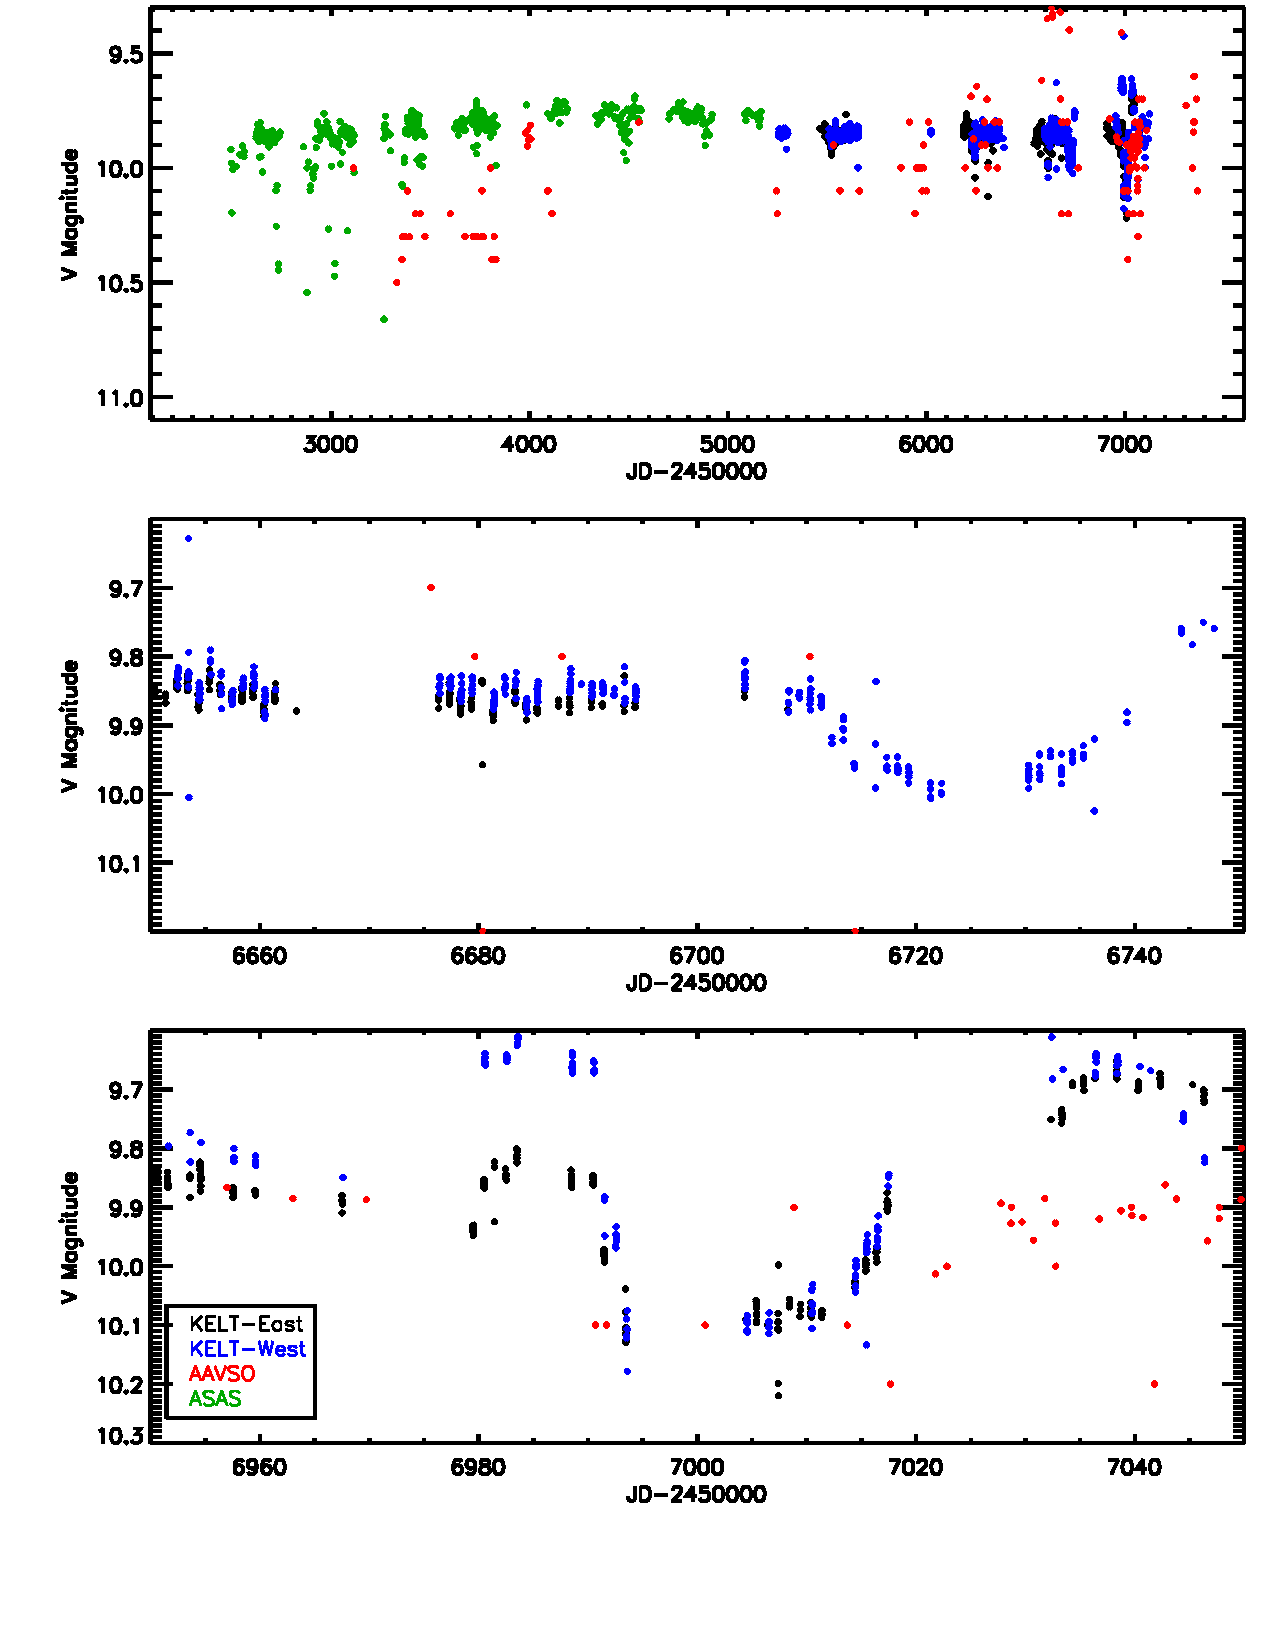
\includegraphics[width=\textwidth]{KELT_eclipses.pdf}
  \figcaption{
 KELT eclipses.
  \label{fig:KELT}}
  \end{center}
\end{figure}

Eclipses \citep{shevchenko92,shevchenko98}.

Eclipse catalog. 

% Table
\begin{deluxetable}{rrrrrl}
% \tabletypesize{font size command}
% \rotate
% \tablewidth{dimen}
% \tablenum{text}
% \tablecolumns{num}
\tablecaption{GW Ori Photometric Eclipse Catolog\label{table:eclipses}}
\tablehead{\colhead{Eclipse Number} & \colhead{JD Start} & \colhead{JD End} & \colhead{Duration} & \colhead{Depth} & \colhead{Telescope}}
\startdata
\nodata & 2456710 & 2456744 & 34 days & 130 mmag & KELT \\
\nodata & 2456989 & 2457030 & $<41$ days & 220 mmag & KELT 
\enddata
\end{deluxetable}

Photometry from KELT (J. Rodriguez) shows that an eclipse happens on JD 6990 - 7020 (+2450000), which corresponds to November 28th, 2014. 

Figure from KELT, ASAS, and AAVSO.

\section{Discussion}

Discussion of our inferred component masses with that of \citet{berger11}. 

Photospheric analysis of properties (based on either spectral type + SED of primary and/or limits on the secondary) coupled with 4 usual PMS models + Choi et al models.

Discussion of component masses relative to ideas about formation, migration.


\section{Notes from 8/17-8/18 meetings}

\subsection{ALMA-related stuff}

- Models of 13CO with a simple structure (vertically isothermal) leave systematic, rotating residuals.  This is a problem we have seen before (see Rosenfeld et al.~2013), and think we understand the origin: a vertical temperature inversion.

- Implemented new model with 5 additional free parameters to describe vertical temperature structure.  (like a sigmoid function).  {Tmid0, qmid, Tatm0, qatm, delta (constant w/ radius), h (previously zq, constant w/ radius)}.  Also allowing gamma to be free.

- New model (probably burned in) fits substantially better than our previous efforts.  Mstars = 5.8 Msun (total).  41.5 degrees inclination (interesting: Mathieu paper has 27 degrees; Berger paper suggests no further than 15 degrees from face-on, very model-dependent; spot modulation in paper by Fang, something also by Bouvier, suggest 35-50 degrees)

- Still seeing bright central peak in systemic velocities in residuals (+/-1.5 km/s).  Need to look better at residuals compared to data.  Might well be real asymmetries...but total dynamical mass seems not to care.


\subsection{Stars}

- The lambda Ori cluster seems to have an age of maybe 5 Myr.  But the GW Ori system has a total mass that implies at least the most massive component is an A/B star.  But it has a G-type spectrum.  That shouldn't be the case unless it is very young (<1 Myr).  So is there an age discrepancy?

- M2sini = 0.11 * (Mtot)$^{2/3}$
- assuming Mtot = 5.5 and coplanar with current disk model, you have M2 = 0.5 Msun.  So M1 = 5.0 Msun.  wtf?  rough estimate of M3sini = 0.1697 * (Mtot)$^{2/3}$, so M3 = 0.85 Msun.

- Max Moe's thesis: B-type stars with T Tauri companions. 

- is GW Ori an x-ray source?

- RV variation of ~8-10 km/s coincides with an eclipse of ~0.6 mags in R, roughly gray.  maybe knife-edge that has asymmetry wrt rotation axis (R-M effect).  

- We are dubious that star 3 can be co-planar with stars A + B and the disk, potentially related to the central residuals that we see.


\subsection{GW Ori as a triple system}

{\it Some notes from Eric from reading literature on what is known about triple systems.  Is this extreme?}

While the ratio between the outer orbital period and the inner orbital period is smaller than in many hierarchical systems, it is not an outlier among triple systems.  In a detailed analysis of higher-order multiple systems, \citet{tokovinin97} found that the ratio $P_{\rm long} / P_{\rm short}$ in almost all systems was greater than 10, presumably reflecting which orbits are stable.  In GW Ori, this ratio is 16.  (!! update with final orbit).  

(Tokovinin has an updated catalog on his website with about twice as many systems as in the CDS version from this paper, but it would be non-trivial to figure out how to remake the above plot.  Not sure it's necessary.)

Among late B star primaries (which GW Ori Aa will be on the main sequence), 13\% of systems have multiplicity of three or higher \citep{eggleton08}; this fraction is roughly constant across spectral types B--G. 

\citet{tokovinin97} finds that the distribution of mutual inclinations of the orbits in triple systems is inconsistent both with complete alignment of the inner and outer orbits, but also with independent inclinations of the two orbits.  However, we should note that this is for a population of much older systems, in which significant dynamical evolution could have occurred, particularly for the shorter-period systems.  The fact that GW Ori appears to have roughly-aligned, circular inner and outer orbits (!! does it?  to be confirmed) is suggestive of formation of one or both companions from the massive disk surrounding the system.  (Wild speculation here.) 

Offner et al 2010 is probably important for us to look at regarding fragmentation vs.\ disk instability.  They also cite Howe \& Clarke 2009 for a review of observations. 

Bate 2012 on his big fragmentation simulation: ``In particular, despite the fact that no objects form closer than $\approx 10$ au from each other, at the end of the calculation there exist 21 binary systems and one triple system with separations $<10$ au.''

In his simulations, of the triples that form, the orbits are misaligned with each other (though three are $\leq 6$ degrees, and 8 out of 9 are $\leq 36$ degrees). 

Bate:  "Observations also indicate that eccentricities e < 0.1 are rare for periods greater than $\approx$ 100 d (separations $\gtrsim$ 1 au). Raghavan et al. (2010) find no binaries with $e < 0.1$ and orbital periods greater than 100 d, though they do find that the outer orbits of two triples and one quadruple have $e < 0.1$. Duquennoy \& Mayor (1991) and Raghavan et al. (2010) also find that the upper-eccentricity envelope is dominated by components of triple systems, possibly due to the action of the Kozai mechanism (Kozai 1962)"

Important for us to see what constraints we have on eccentricity of the orbits. 


\section{huh}


Orbit calculation \citep{mathieu91}.

H-band interferometry, resolved orbit \citep{berger11}.

Spectroscopic activity and inner disk clearing \citep{fang14}.


\section{Observations and Data Reduction -- {\bf Ian, Sean, David L.}}\label{sec:data}


\section{CO Modeling and Results -- {\bf Ian, Sean}} \label{sec:method}



\section{Discussion -- {\bf Eric, Willie, Keivan}}\label{sec:disc}



\subsection{Comparison to Previous Results}

\subsection{Comparison to Pre-MS Evolution Models}


\section{Summary and Conclusions -- {\bf Ian, Sean, Keivan, Eric, Willie}} \label{sec:summary}

We have analyzed ALMA observations of the XX transitions from the GW Ori circumtriple disk.  The main conclusions of this work include: \\

\noindent $\bullet$ The mass is XX.


\acknowledgments
IC is supported by the Smithsonian Institution. IC acknowledges helpful conversations with Maxwell Moe about GW Ori and related systems.  SA acknowledges the very helpful support provided by the NRAO Student Observing Support program related to the early development of this project.  This paper makes use of the following ALMA data: XX  ALMA is a partnership of ESO (representing its member states), NSF (USA), and NINS (Japan), together with NRC (Canada) and NSC and ASIAA (Taiwan), in cooperation with the Republic of Chile.  The Joint ALMA Observatory is operated by ESO, AUI/NRAO, and NAOJ.  This research made extensive use of the Julia programming language \citep{julia12} and Astropy \citep{astropy13}.

\begin{thebibliography}{}

\bibitem[Alencar et al.(2003)]{alencar03} Alencar, S.~H.~P., Melo, C.~H.~F., Dullemond, C.~P., Andersen, J., Batalha, C., Vaz, L.~P.~R., \& Mathieu, R.~D.\ 2003, \aap, 409, 1037 

\bibitem[Allard et al.(2003)]{allard03} Allard, F., Guillot, T., 
Ludwig, H.-G., et al.\ 2003, Brown Dwarfs, 211, 325 

\bibitem[Andersen et al.(1989)]{andersen89} Andersen, J., Lindgren, H., Hazen, M.~L., \& Mayor, M.\ 1989, \aap, 219, 142

\bibitem[Andrews et al.(2013)]{andrews13} Andrews, S.~M., Rosenfeld, K.~A., Kraus, A.~L., \& Wilner, D.~J.\ 2013, \apj, 771, 129

\bibitem[Anthonioz et al.(2015)]{anthonioz15} Anthonioz, F., M{\'e}nard, F., Pinte, C., et al.\ 2015, \aap, 574, A41 

\bibitem[Astropy Collaboration(2013)]{astropy13} Astropy Collaboration 2013,
  \href{http://dx.doi.org/10.1051/0004-6361/201322068}, \aap,
  558, 33
  
\bibitem[Baraffe et al.(2015)]{baraffe15} Baraffe, I., Homeier, D., Allard, F., \& Chabrier, G.\ 2015, arXiv:1503.04107 

\bibitem[Berger et al.(2011)]{berger11} Berger, J.-P., Monnier, J.~D., Millan-Gabet, R., et al.\ 2011, \aap, 529, L1 

\bibitem[Bessell(1979)]{bessell79} Bessell, M.~S.\ 1979, \pasp, 91, 589 

\bibitem[Bezanson et~al.(2012)]{julia12} Bezanson, J., Karpinski, S., Shah, V.~B., \& Edelman, A.\ 2012, ArXiv e-prints,
  \href{http://arxiv.org/abs/1209.5145}{{\sffamily arXiv:1209.5145 [cs.PL]}}

\bibitem[Casagrande et al.(2010)]{casagrande10} Casagrande, L., Ram{\'{\i}}irez, I., Mel{\'e}ndez, J., Bessell, M., \& Asplund, M.\ 2010, \aap, 512, 54

\bibitem[Dotter et al.(2008)]{dotter08} Dotter, A., Chaboyer, B., Jevremovi{\'c}, D.\ et al.\ 2008, \apjs, 178, 89

\bibitem[Eggleton 
\& Tokovinin(2008)]{eggleton08} Eggleton, P.~P., \& Tokovinin, A.~A.\ 2008, \mnras, 389, 869 


\bibitem[Fabrycky et al.(2014)]{fabrycky14} Fabrycky, D.~C., Lissauer, J.~J., Ragozzine, D., et al.\ 2014, \apj, 790, 146 

\bibitem[Fang et al.(2014)]{fang14} Fang, M., Sicilia-Aguilar, A., Roccatagliata, V., et al.\ 2014, \aap, 570, A118 

\bibitem[Figueira et al.(2012)]{figueira12} Figueira, P., Marmier, M., Bou{\'e}, G., et al.\ 2012, \aap, 541, A139 

\bibitem[Fitzpatrick(1999)]{fitzpatrick99} Fitzpatrick, E.~L.\ 1999, 
\pasp, 111, 63 

\bibitem[Foreman-Mackey et al.(2013)]{foreman-mackey13} Foreman-Mackey, D., Hogg, D.~W., Lang, D., \& Goodman, J.\ 2013, \pasp, 125, 306

\bibitem[{Foreman-Mackey {et~al.}(2014)Foreman-Mackey, Price-Whelan, Ryan,
  Rice, Smith, Barbary, Hogg, \& Brewer}]{foreman-mackey14}
Foreman-Mackey, D., Price-Whelan, A., Ryan, G., {et~al.}
  \href{http://dx.doi.org/10.5281/zenodo.10598}{2014}

\bibitem[{Frigo \& Johnson(2005)}]{fftw}
Frigo, M., \& Johnson, S.~G. 2005, Proceedings of the IEEE, 93,
  216, special issue on ``Program Generation, Optimization, and Platform
  Adaptation''

\bibitem[{Gelman {et~al.}(2013)Gelman, Carlin, Stern, Dunson, Vehtari, \&
  Rubin}]{gelman13}
Gelman, A., Carlin, J., Stern, H., {et~al.} 2013, {Bayesian Data Analysis,
  Third Edition}, {Chapman \& Hall/CRC Texts in Statistical Science} (Taylor \&
  Francis)

\bibitem[Gennaro et al.(2012)]{Gennaro2012} Gennaro, M., Prada Moroni, P.~G., \& Tognelli, E.\ 2012, \mnras, 420, 986

\bibitem[G{\'o}mez de Castro(2009)]{castro09} G{\'o}mez de Castro, A.~I. 2009, \apj, 698, L108

\bibitem[G{\'o}mez de Castro et al.(2013)]{castro13} G{\'o}mez de Castro, A.~I., L{\'o}pez-Santiago, J., Talavera, A., Sytov, A.~Y., \& Bisikalo, D. 2013, \apj, 766, 62

\bibitem[G{\'o}mez Maqueo Chew et al.(2012)]{Gomez2012} G{\'o}mez 
Maqueo Chew, Y., Stassun, K.~G., Pr{\v s}a, A., et al.\ 2012, \apj, 745, 58

\bibitem[Gray(1992)]{gray92} Gray, D.~F.\ 1992, The Observation and Analysis of Stellar Photospheres (Cambridge: Cambridge Univ.~Press)

\bibitem[Guilloteau et 
al.(2014)]{guilloteau14} Guilloteau, S., Simon, M., Pi{\'e}tu, V., et al.\ 2014, \aap, 567, A117 
  
\bibitem[Hillenbrand \& White(2004)]{Hillenbrand2004} Hillenbrand, L.~A., \& White, R.~J.\ 2004, \apj, 604, 741
  
\bibitem[Jensen \& Mathieu(1997)]{jensen97} Jensen, E.~L.~N., \& Mathieu, R.~D.\ 1997, \aj, 114, 301 

\bibitem[J{\o}rgensen \& Lindegren(2005)]{jorgensen05} J{\o}rgensen, B.~R., \& Lindegren, L.\ 2005, \aap, 436, 127 

\bibitem[Lynden-Bell \& Pringle(1974)]{lynden-bell74} Lynden-Bell, D., \& Pringle, J.~E.\ 1974, \mnras, 168, 603

\bibitem[Manset et al.(2005)]{manset05} Manset, N., Bastien, P., 
\& Bertout, C.\ 2005, \aj, 129, 480 

\bibitem[Marino et al.(2015)]{marino15} Marino, S., Perez, S., Casassus, S.\ 2015, \apj, 798, L44

\bibitem[Mathieu et al.(1991)]{mathieu91} Mathieu, R.~D., Adams, 
F.~C., \& Latham, D.~W.\ 1991, \aj, 101, 2184 

\bibitem[Mathieu et al.(2007)]{Mathieu2007} Mathieu, R.~D., 
Baraffe, I., Simon, M., Stassun, K.~G., 
\& White, R.\ 2007, Protostars and Planets V, 411 (University of Arizona Press, Tucson)

\bibitem[Mathis(1990)]{mathis90} Mathis, J.~S.\ 1990, \araa, 28, 37

\bibitem[Pavlyuchenkov et al.(2007)]{pavlyuchenkov07} Pavlyuchenkov, Y., Semenov, D., Henning, T., Guilloteau, S., Pi{\'e}tu, V., Launhardt, R., \& Dutrey, A.\ 2007, \apj, 669, 1262

\bibitem[Pecaut et al.(2012)]{pecaut12} Pecaut, M.~J., Mamajek, 
E.~E., \& Bubar, E.~J.\ 2012, \apj, 746, 154 

\bibitem[Pecaut \& Mamajek(2013)]{pecaut13} Pecaut, M.~J., \& Mamajek, E.~E.\ 2013, \apjs, 208, 9

\bibitem[Perryman et al.(1997)]{perryman97} Perryman, M.~A.~C., Lindegren, L., Kovalevsky, J., et al.\ 1997, \aap, 323, L49 

\bibitem[Pi{\'e}tu et al.(2007)]{pietu07} Pi{\'e}tu, V., Dutrey, A., \& Guilloteau, S.\ 2007, \aap, 467, 163

\bibitem[Popper(1980)]{popper80} Popper, D.~M.\ 1980, \araa, 18, 115

\bibitem[Rosenfeld et al.(2012a)]{rosenfeld12b} Rosenfeld, K.~A., Qi, C., Andrews, S.~M., et al.\ 2012, \apj, 757, 129 

\bibitem[Rosenfeld et al.(2012b)]{rosenfeld12} Rosenfeld, K.~A., Andrews, S.~M., Wilner, D.~J., \& Stempels, H.~C.\ 2012, \apj, 759, 119 (2012b)

\bibitem[Rosenfeld et~al.(2014)]{rosenfeld14} Rosenfeld, K.~A., Chiang, E., \& Andrews, S.~M.\ 2014, \apj, 782, 62
  
\bibitem[Schaefer et~al.(2009)]{schaefer09} Schaefer, G.~H., Dutrey, A., Guilloteau, S., Simon, M., \& White, R.~J. 2009, \apj, 701, 698

\bibitem[{{Schwab}(1984)}]{schwab84}
{Schwab}, F.~R. 1984, in {Indirect Imaging. Measurement and Processing for
  Indirect Imaging}, ed. J.~A. {Roberts}, 333 (Cambridge: Cambridge Univ.~Press)

\bibitem[Shevchenko et al.(1992)]{shevchenko92} Shevchenko, V.~S., 
Grankin, K.~N., Ibragimov, M.~A., 
\& Melnikov, S.~Y.\ 1992, Information Bulletin on Variable Stars, 3746, 1 

\bibitem[Shevchenko et al.(1998)]{shevchenko98} Shevchenko, V.~S., 
Grankin, K.~N., Mel'Nikov, S.~Y., 
\& Lamzin, S.~A.\ 1998, Astronomy Letters, 24, 528 


\bibitem[Simon et al.(2000)]{simon00} Simon, M., Dutrey, A., \& Guilloteau, S.\ 2000, \apj, 545, 1034

\bibitem[Siess et al.(2000)]{siess00} Siess, L., Dufour, E., \& Forestini, M.\ 2000, \aap, 358, 593 

\bibitem[Stassun et al.(2004)]{Stassun2004} Stassun, K.~G., 
Mathieu, R.~D., Vaz, L.~P.~R., Stroud, N., 
\& Vrba, F.~J.\ 2004, \apjs, 151, 357 

\bibitem[Stassun et al.(2006)]{Stassun2006} Stassun, K.~G., 
Mathieu, R.~D., \& Valenti, J.~A.\ 2006, \nat, 440, 311 

\bibitem[Stassun et al.(2007)]{Stassun2007} Stassun, K.~G., 
Mathieu, R.~D., \& Valenti, J.~A.\ 2007, \apj, 664, 1154

\bibitem[Stassun et al.(2008)]{Stassun2008} Stassun, K.~G., 
Mathieu, R.~D., Cargile, P.~A., et al.\ 2008, \nat, 453, 1079 

\bibitem[Stassun et al.(2014)]{Stassun2014} 
Stassun, K.~G., Feiden, G.~A., \& Torres, G.\ 2014, New Astron. Rev., 60, 1

\bibitem[Tognelli et al.(2011)]{tognelli11} Tognelli, E., Prada Moroni, P.~G., \& Degl'Innocenti, S.\ 2011, \aap, 533, AA109 

\bibitem[Tokovinin(1997)]{tokovinin97} Tokovinin, A.~A.\ 1997, \aaps, 124, 75 


\bibitem[Tremaine \& Dong(2012)]{tremaine12} Tremaine, S., \& Dong, S.\ 2012, \aj, 143, 94

\bibitem[van Leeuwen(2007)]{vanleeuwen07} van Leeuwen, F.\ 2007, \aap, 474, 653


\end{thebibliography}


\begin{figure*}[htb]
\begin{center}
  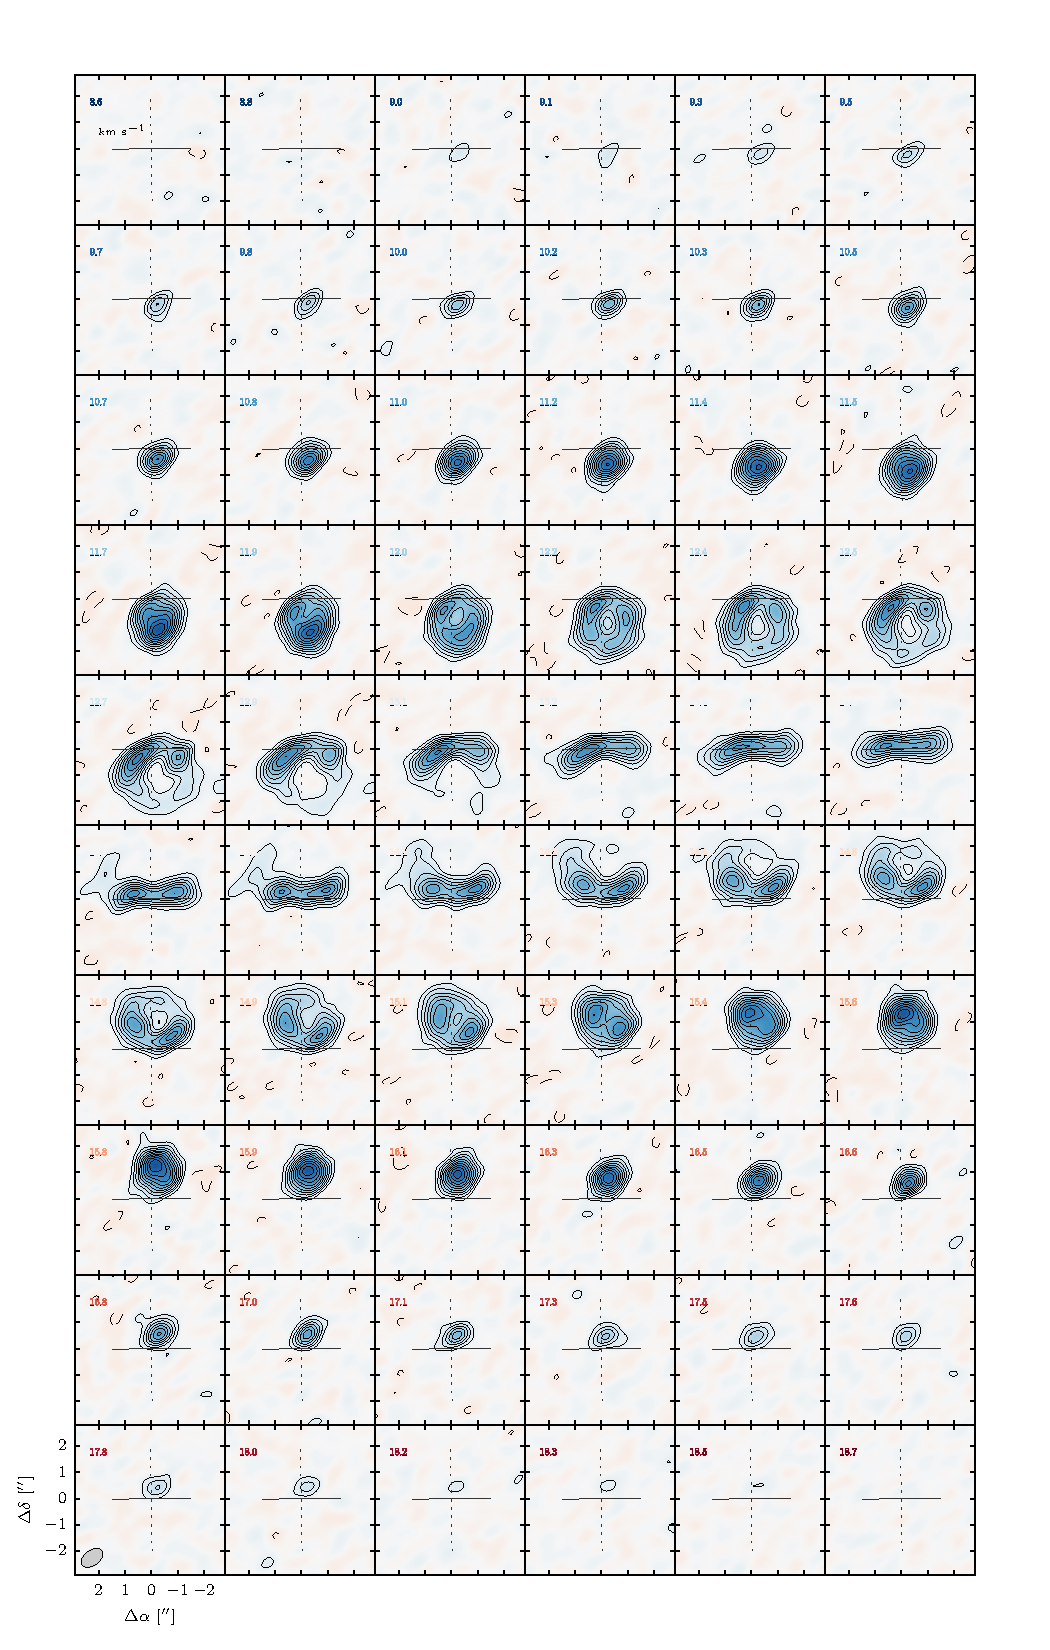
\includegraphics[height=9in]{13CO_iso_data.pdf}
  \figcaption{Channel maps for the isothermal 13CO data.
  \label{fig:13CO_isothermal}}
  \end{center}
\end{figure*}

\begin{figure*}[htb]
\begin{center}
  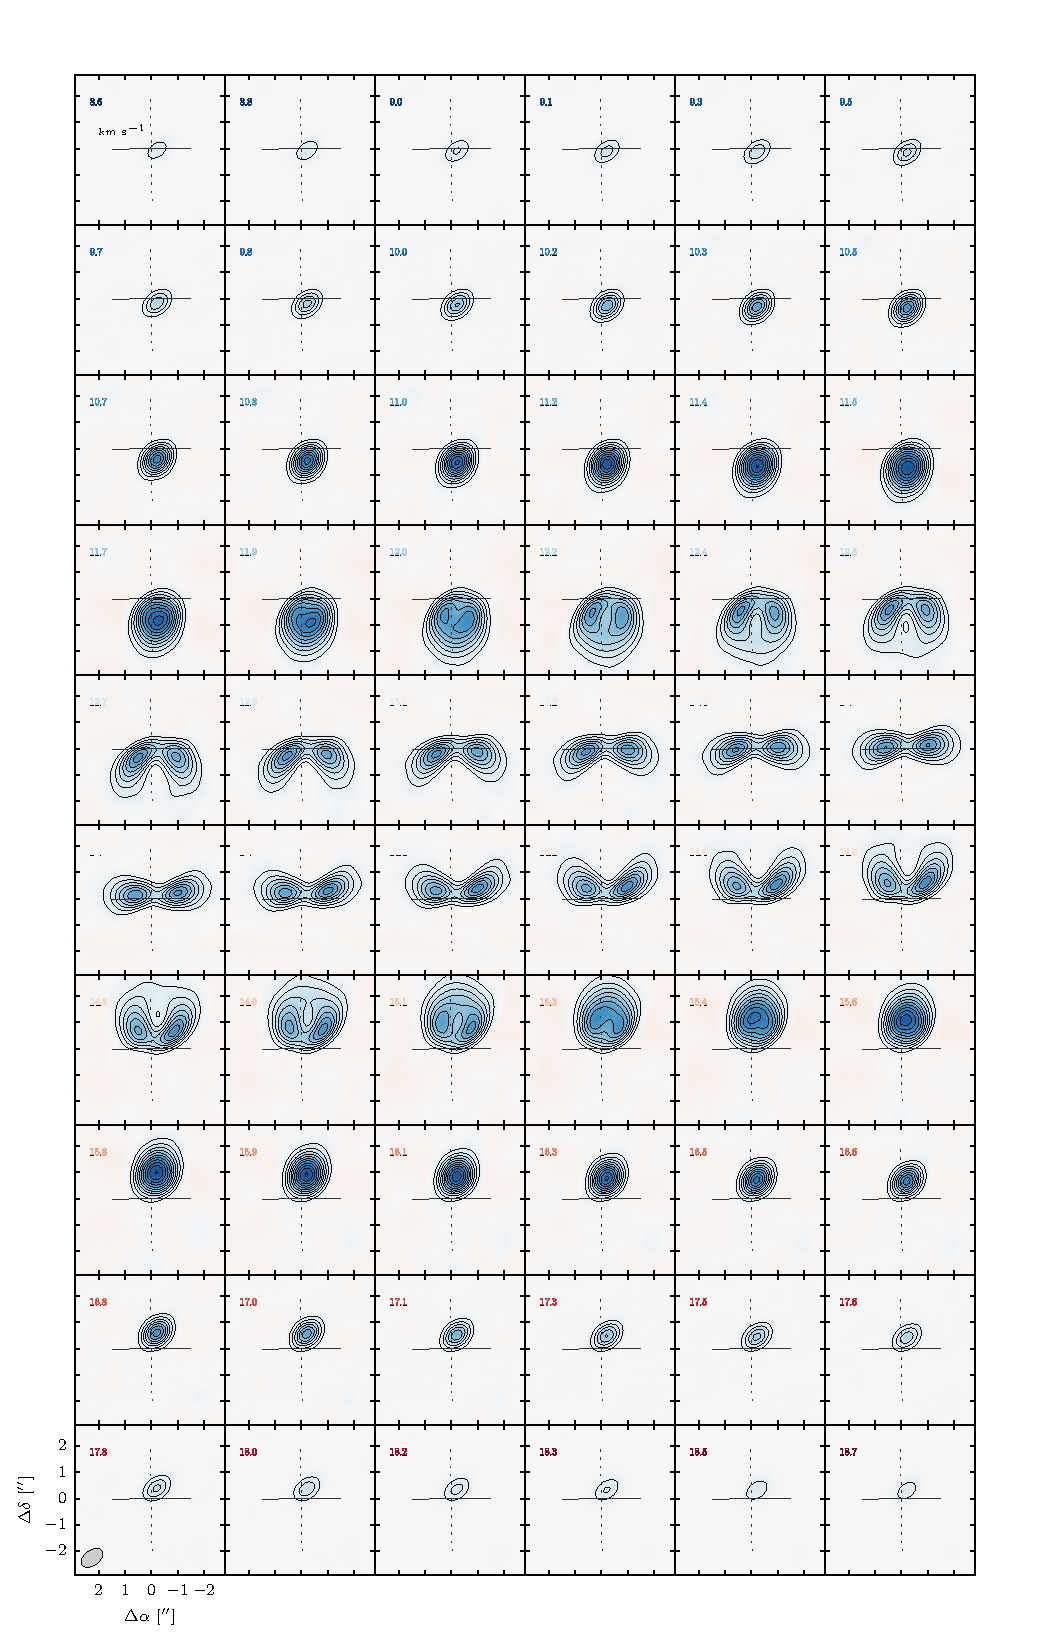
\includegraphics[height=9in]{13CO_iso_model.pdf}
  \figcaption{Channel maps for the isothermal 13CO model.
  \label{fig:13CO_isothermal_model}}
  \end{center}
\end{figure*}

\begin{figure*}[htb]
\begin{center}
  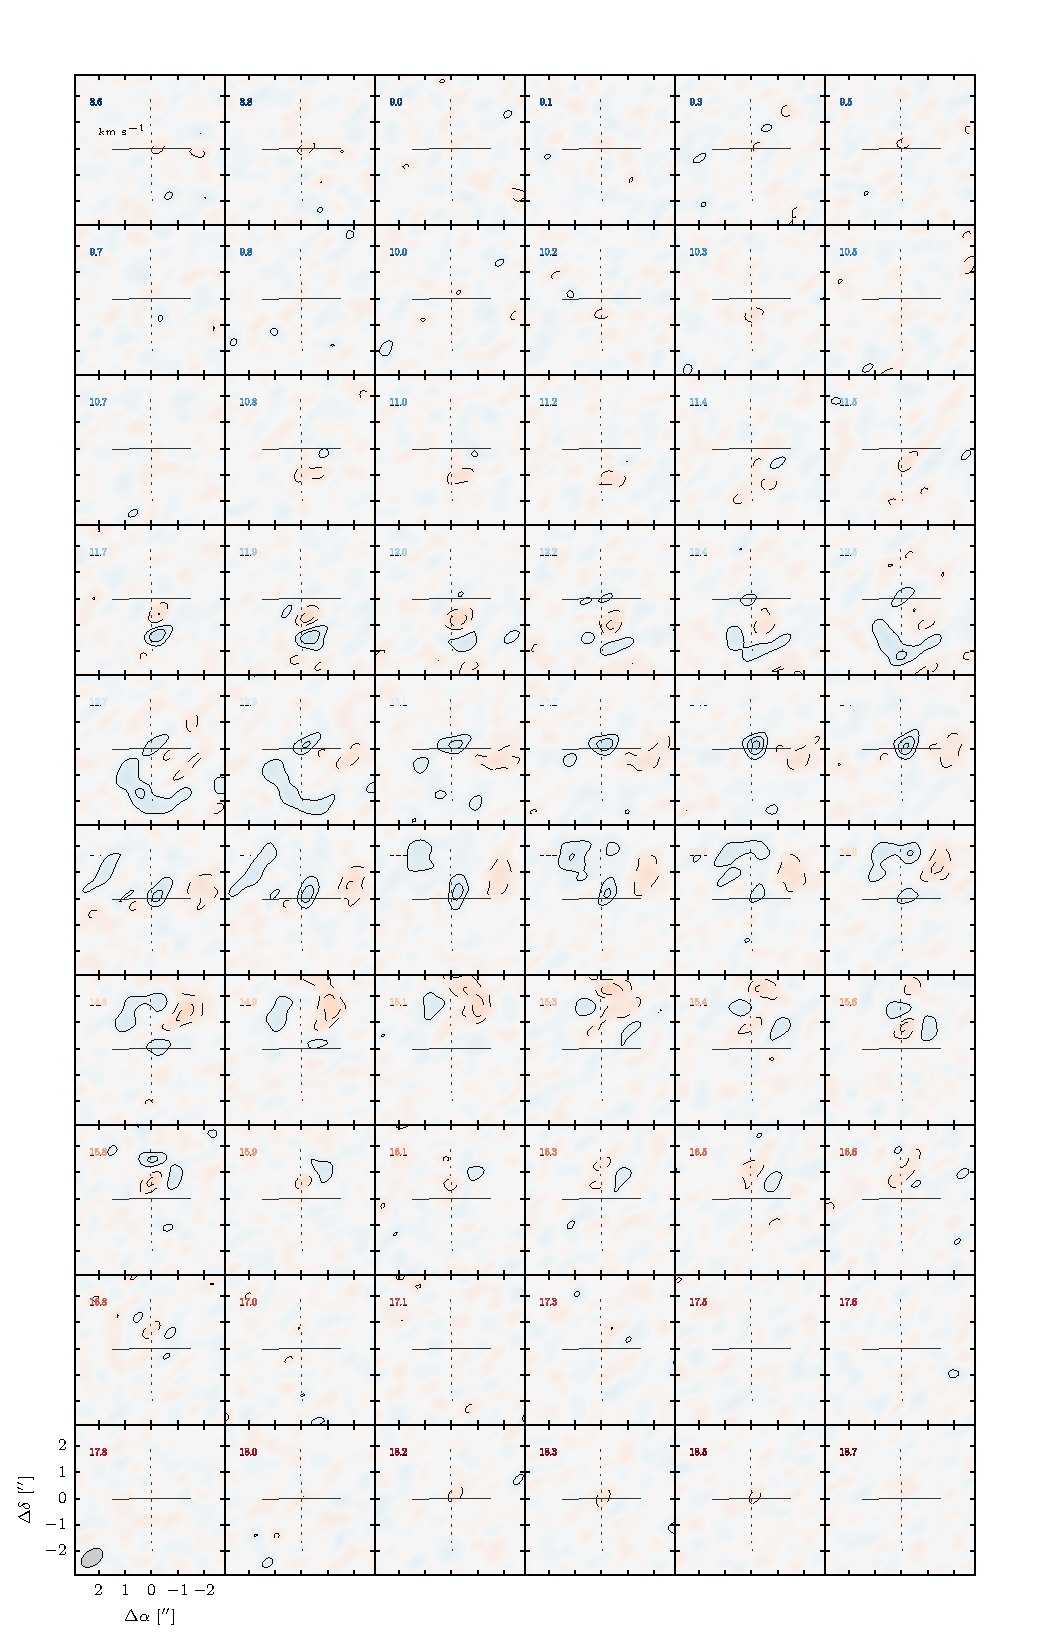
\includegraphics[height=9in]{13CO_iso_resid.pdf}
  \figcaption{Channel maps for the isothermal 13CO residuals. Residuals related to a vertical temperature gradient are seen.
  \label{fig:13CO_isothermal_resid}}
  \end{center}
\end{figure*}


\begin{figure*}[htb]
\begin{center}
  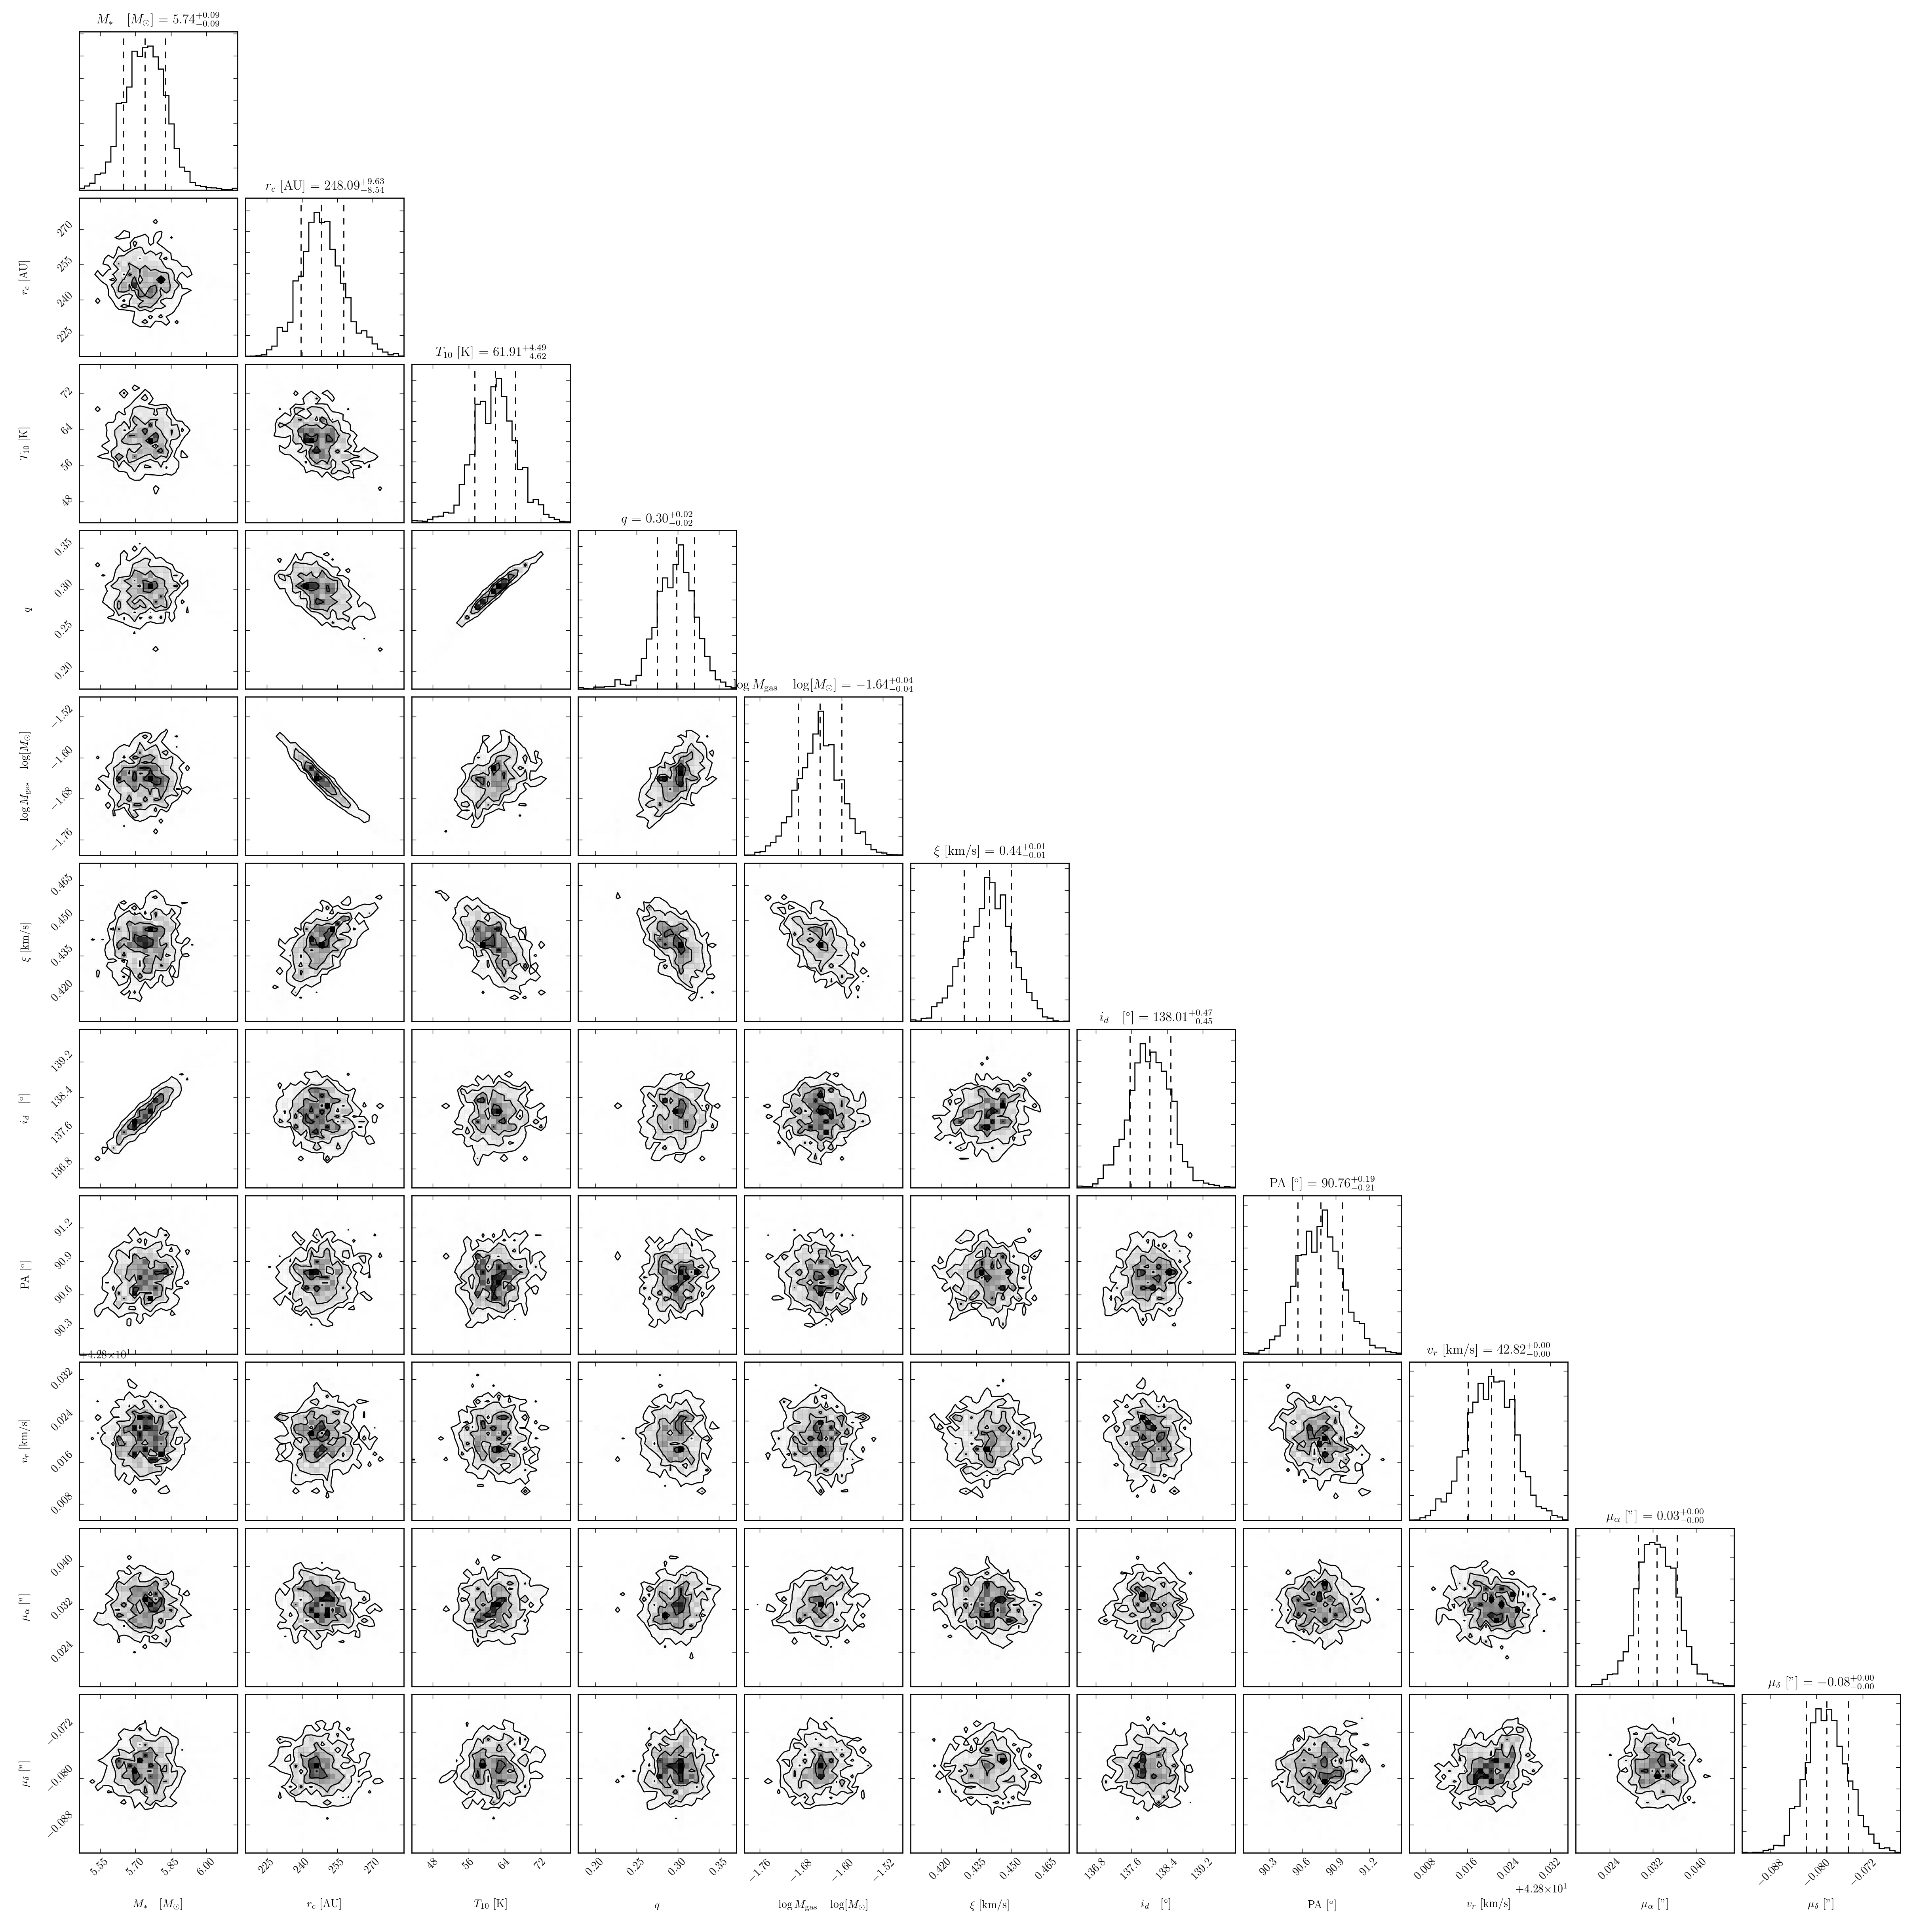
\includegraphics[width=6in]{13CO_iso_triangle.png}
  \figcaption{Posterior for the isothermal 13CO residuals.
  \label{fig:13CO_iso_triangle}}
  \end{center}
\end{figure*}



\end{document}
